%Dies ist die Hauptseite des Dokumentes. Es werden u. a. alle Kapitel,
%Einstellung im Header eingebunden.
%Veränderungen müssen in folgenden Dateien vorgenommen werden:
      %- config.tex
      %- Versionsübersicht
      %- einzelne Kapitel (evtl. erweitern)

\input{common/layout.tex}          % Diese Datei enthält alle
                                          % Layouteinstellungen
\newcommand{\dokumentTitel}{Testspezifikation}
% Definition von globalen Parametern, die derzeit auf der Titelseite und in der
% Kopfzeile verwendet werden. Der in <> gesetzte Text ist zu verändern.

\newcommand{\praktikumTitel}{<Titel des Praktikums>}
\newcommand{\projektTitel}{<Titel des Teilprojektes>}
\newcommand{\institut}{
	<Name des Instituts>\\
	<Name des Institutsleiters>\\
	<Straße und Hausnummer>\\
	<Postleitzahl und Ort>\\
}
\newcommand{\institutsLogo}{common/ISF_Logo.pdf}
\newcommand{\betreuer}{<Name>}

\externaldocument{Pflichtenheft}
\externaldocument{Systementwurf}

%------Beginn des Gesamtdokumentes----------------------------------------------
\begin{document}

%------Eingebundene Seiten, Verzeichnisse bzw. Kapitel--------------------------
\include{common/titelseite}                      % Titelseite
%!TEX root = ../Testspezifikation.tex

%----\"Uberschrift------------------------------------------------------------
{\relsize{2}\textbf{Versions\"ubersicht}}\\[2ex]

%----Start der Tabelle------------------------------------------------------
\begin{longtable}{|m{1.78cm}|m{1.59cm}|m{2.86cm}|m{1.9cm}|m{5.25cm}|}

  \hline                                              % Linie oberhalb

  %----Spalten\"uberschriften------------------------------------------------
  \textbf{Version}  &    \textbf{Datum}  &    \textbf{Autor(en)}  &
  \textbf{Status}   &    \textbf{Kommentar}  \\       %Spalten\"uberschrift
  \hline                                              % Gitterlinie

  %----die nachfolgeden beiden Zeilen so oft wiederholen und die ... mit den
  %i   entsprechenden Daten zu f\"ullen wie erforderlich
  0.1    &    28.04.2014    &    P. Dittrich    &        &   
  Einleitung und Testplan, sowie Komponentendiagramm eingefügt\\
  \hline                                              % Gitterlinie unten
  0.2    &    01.05.2014    &    F. Heymann    &        &   
  Kapitel 2.2, 2.3, 2.4, 2.5 hinzugefügt\\
  \hline                                              % Gitterlinie unten
  0.3    &    02.05.2014    &    N. Widdecke    &        &   
  Kapitel 3 hinzugefügt\\
  \hline
  0.4    &    02.05.2014    &    C. Sontag    &        &   
  Kapitel 3.3.1 hinzugefügt\\
  \hline  
  0.5    &    02.05.2014    &    P. Dittrich    &        &   
  Kapitel 3.2 hinzugefügt und 3.1 bearbeitet\\
  \hline
  0.6    &    03.05.2014    &    D. Klose    &        &   
  Kapitel 3.3.3 Test-Case <T201> bearbeitet\\
  \hline  
  0.7    &    03.05.2014    &    A. Reiss    &        &   
  Kapitel 3.3.2 Test-Case <T200> bearbeitet\\
  \hline  
  0.8    &    05.05.2014    &    Auftragnehmer    &        &   
  diverse Verbesserungen\\
  \hline
  1.0    &    05.05.2014    &    Auftragnehmer    &    vorläufig    &   
  Hinweise des Betreuers eingearbeitet\\
  \hline 
  1.1    &    16.07.2014    &    C. Sontag    &        &   
  Unit-Tests hinzugefügt\\
  \hline 
%----Ende der Tabelle------------------------------------------------------
\end{longtable}

%Status: "`in Bearbeitung"', "`vorgelegt"', "`vorläufig"', "`abgenommen"' oder "`abgelehnt"'\\
%Kommentar: hier eintragen, was und wo geändert bzw. ergänzt wurde (z.B. Kapitel )

       % Versionsübersicht

\tableofcontents                          % Inhaltsverzeichnis wird automatisch
                                          % generiert
\listoffigures                            % ebenso das Abbildungsverzeichnis

%----Kapitel des Feinentwurfs, die mit Inhalt zu füllen sind--------------------
\chapter{Einleitung}

Hier soll kurz das Ziel dieses Dokumentes beschrieben werden.

%!TEX root = ../Testspezifikation.tex

\chapter{Testplan}

Im Folgenden wird der Testplan für \NewsGenie erläutert. Einzelne Komponenten
und ihre Funktionsweise, sowie die daraus resultierende Teststrategie werden
vorgestellt. 

\NewsGenie setzt mit Sprachsteuerung auf ein Eingabemedium, für das dem Benutzer
keine eigenen Strategien zur Fehlerbehandlung zur Verfügung stehen (am
Bildschirm zum Beispiel das Schließen und erneute Öffnen des Programms),
deshalb muss besonderes Augenmerk auf die Stabilität, Fehlertoleranz und einfache
Bedienbarkeit dieser Schnittstelle gelegt werden.

\section{Zu testende Komponenten}

\NewsGenie wird aus einem Client und verschiedenen Serverkomponenten bestehen.
Wie in Abb. \ref{komponenten} dargestellt handelt es sich dabei um

\begin{description}
\item[Client] Läuft auf einem Raspberry Pi Einplatinencomputer und
wird die direkte Interaktion mit dem Benutzer übernehmen, sowie dessen Anfragen
an den Server weiterleiten
\item[Crawler] Eine Serveranwendung, die im Hintergrund die vom Benutzer
hinzugefügten RSS-Feeds durchsucht und indexiert. Bereitet die Daten für den
QueryProcessor auf.
\item[QueryProcessor] Nimmt die Anfragen der Clients entgegen und generiert
möglichst präzise Antworten auf die gestellten Fragen. Dabei greift er auf die
vom Crawler indexierten Daten zu.
\item[Webinterface] Ist für die Registrierung und die Einstellungen der Nutzer
zuständig. Außerdem bietet das Webinterface Funktionen zur textbasierten Anfrage
des QueryProcessors.
\item[Datenbank] Verbindet die einzelnen Komponenten und muss deshalb ein
robustes Schema bieten, auf das alle Anwendungen gleichzeitig zugreifen können.
\end{description}

\begin{figure}[h]
\centering
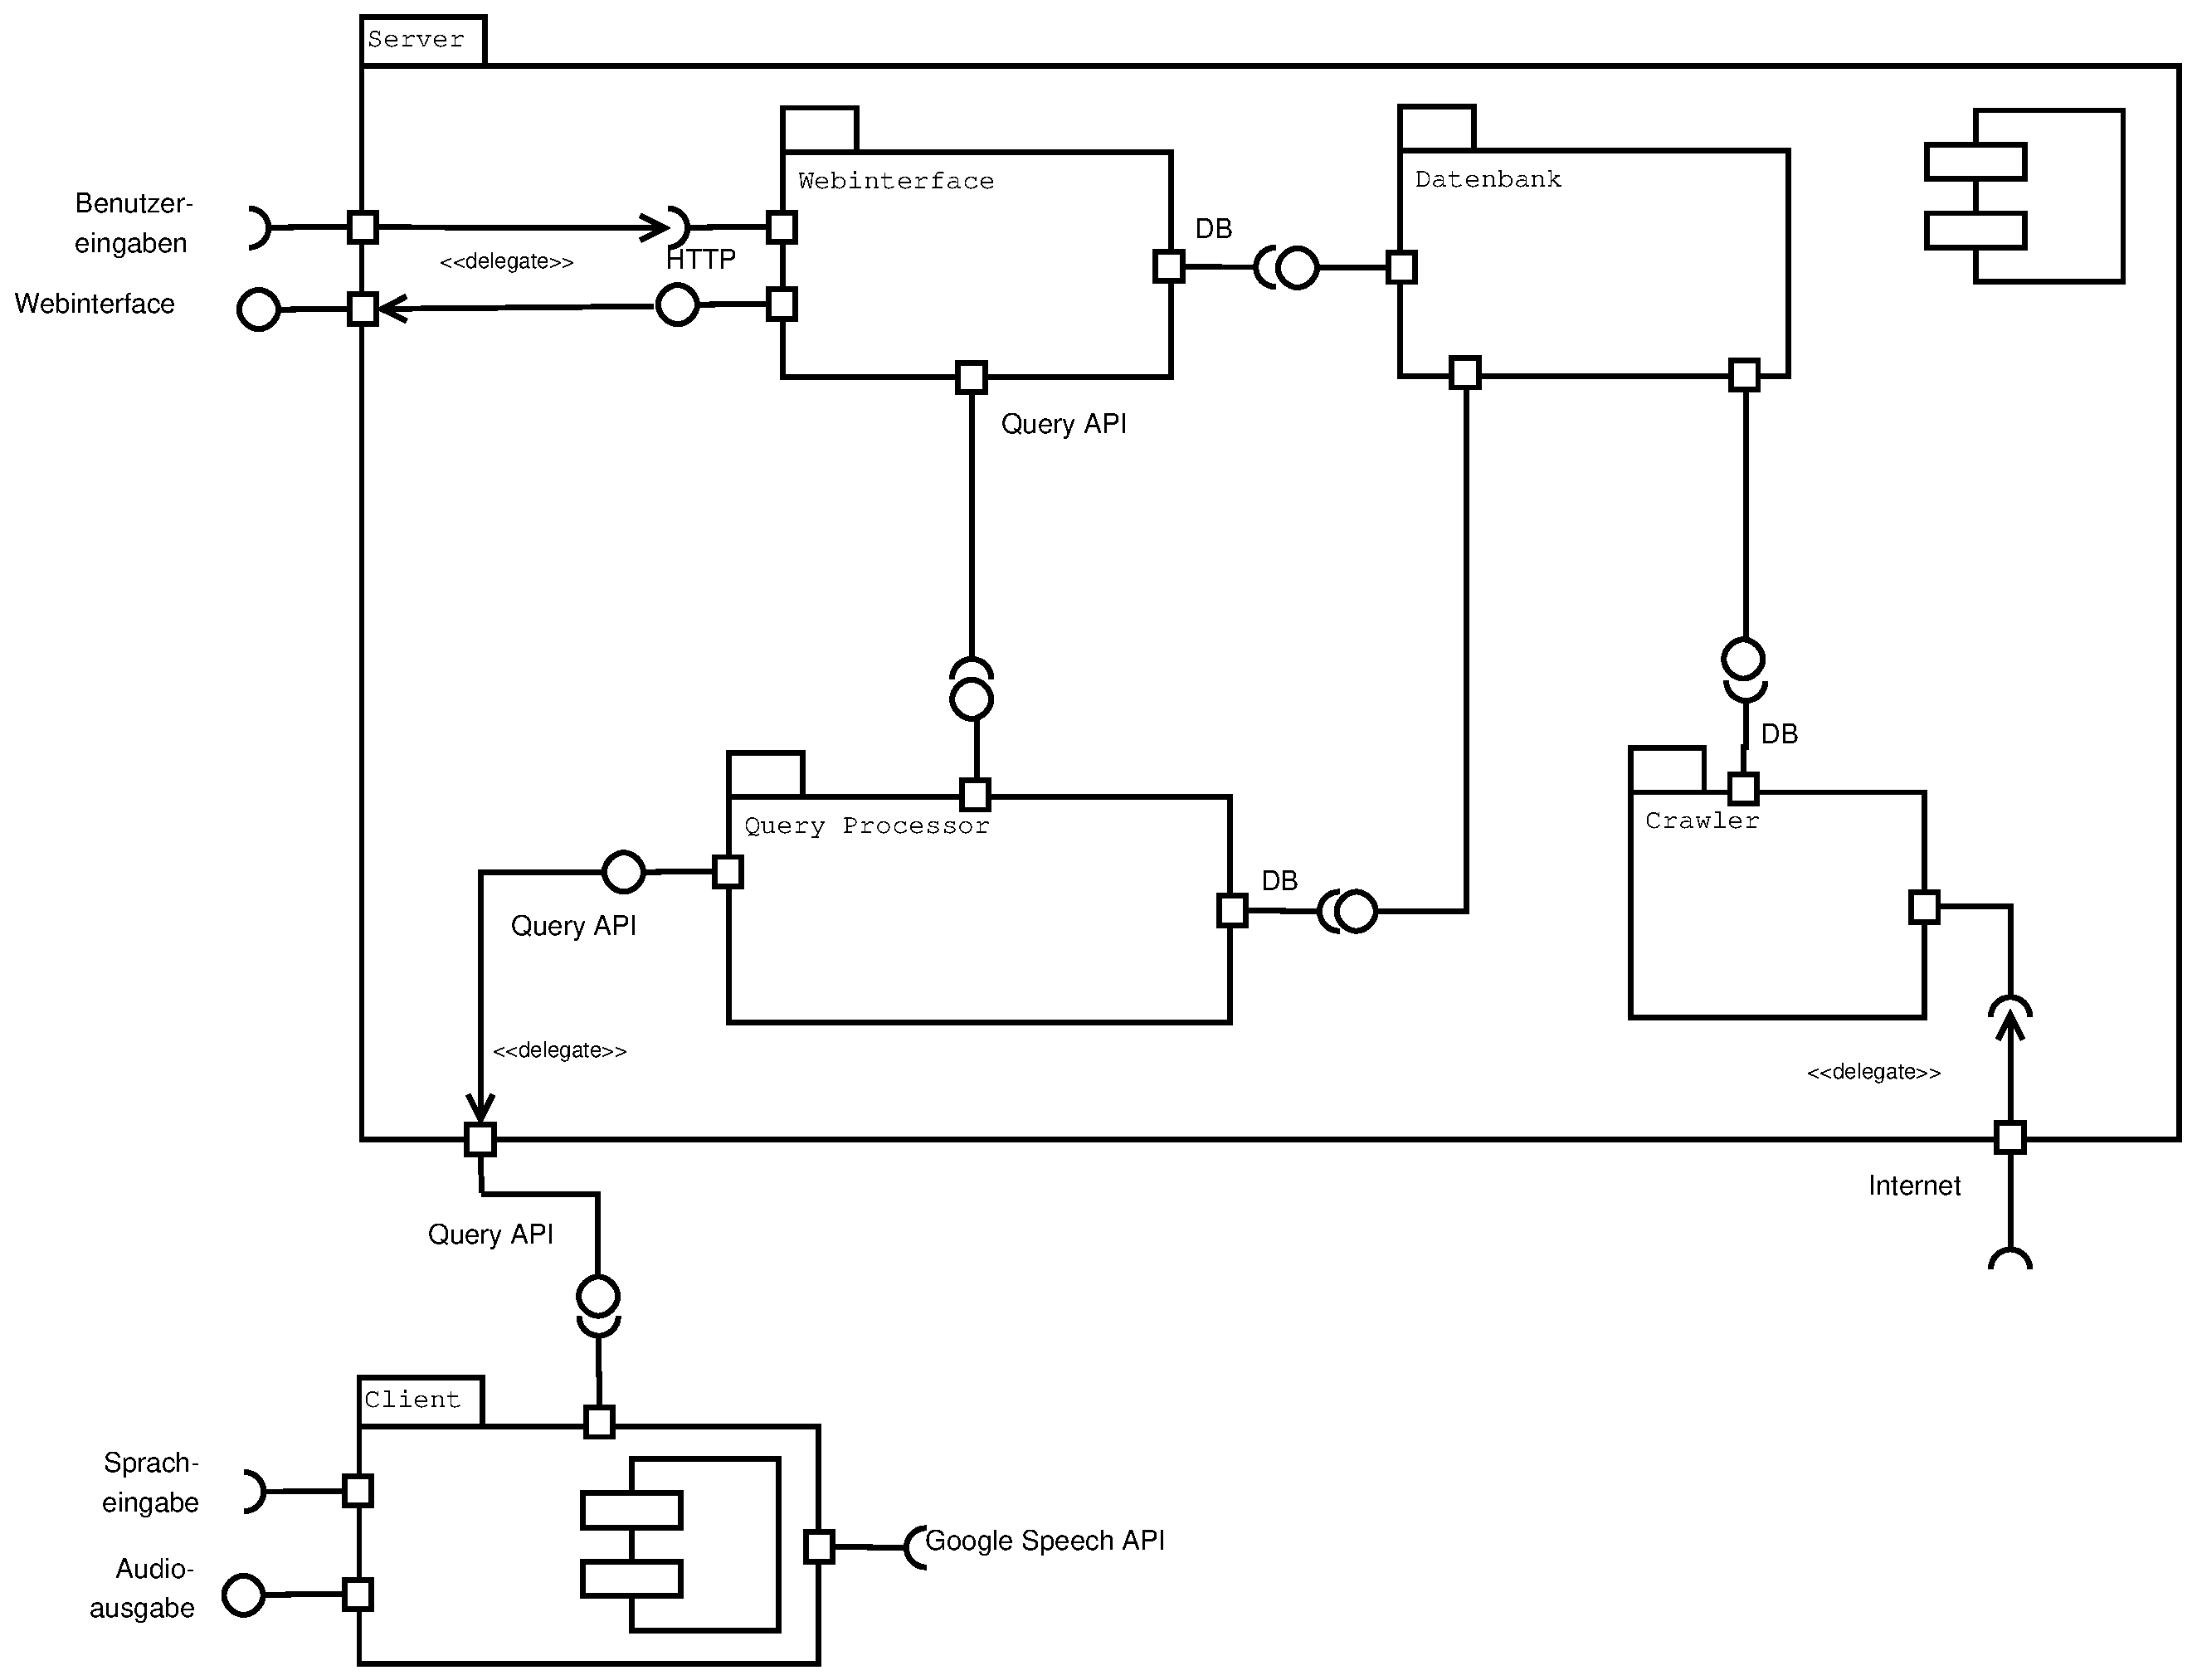
\includegraphics[width=1\textwidth]{Testspezifikation/testplan/komponenten}
\caption{Komponentendiagramm, \textit{Architektur von \NewsGenie}
\label{komponenten}}
\end{figure}

\pagebreak
\section{Zu testende Funktionen/Merkmale}

\begin{itemize}
\item \ref{RM1} Ein- und Ausgabe in natürlicher Sprache:  Das System ist in der Lage verbal mit dem Benutzer zu kommunizieren.
Um dies zu ermöglichen, kann es gesprochene Anfragen aufnehmen und verarbeiten sowie Antworten formulieren und leicht verständlich ausgeben.
\item \ref{RM2} Interaktives Verhalten: Das System grenzt Anfragen mit Ja-/Nein-Fragen ein, bricht die Sprachausgabe bei einem Stopp-Befehl ab und erlaubt negatives Feedback.
\item \ref{RM4} Benutzerschnittstelle: Das Webinterface bietet die Möglichkeit, Textanfragen zu stellen und die Resultate manuell zu validieren.
\item \ref{RM5} Backend: Nachrichtendaten werden in einem \glqq Triplestore\grqq\ mit \glqq Inverted Indexes\grqq\ gespeichert um effiziente Volltextsuche zu ermöglichen. Zu einer Anfrage werden ausschließlich dazu passende Artikel ausgegeben.
\item \ref{F10} Ausgabe von natürlicher Sprache: Der Client kann natürliche Sprache ausgeben.
\item \ref{F11} Aufnahme von natürlicher Sprache: Der Client kann natürliche Sprache aufnehmen.
\item \ref{F12} Umwandlung von Sprache in Text: Das System kann Sprachdateien in Text umwandeln.
\item \ref{F13} Umwandlung von Text in Sprache: Das System kann Text in Sprachdateien umwandeln.
\item \ref{F30}, \ref{F20} Anfrage stellen: Wenn der Benutzer am Client eingeloggt ist, kann er Anfragen stellen und erhält eine sinnvolle Antwort.
\item \ref{F30} Client Login: Ein Benutzer kann sich am Client einloggen.
\item \ref{F30}, \ref{F31} Client Logout: Nach einem Login am Client kann sich ein Benutzer wieder ausloggen.
\item \ref{F40} News-Crawling: Neue Artikel werden regelmäßig in das System aufgenommen.
\item \ref{F50} Registrierung: Neue Benutzer können sich registrieren.
\item \ref{F60} Webinterface Login: Benutzer können sich am Webinterface einloggen.
\item \ref{F60}, \ref{F61} Webinterface Logout: Nach einem Login am Webinterface kann sich ein Benutzer wieder ausloggen.
\item \ref{F60}, \ref{F70} Feed-Liste anzeigen: Eingeloggten Benutzern wird eine Liste ihrer abonnierten Feeds angezeigt.
\item \ref{F60}, \ref{F71} Feed hinzufügen: Eingeloggte Benutzer können neue Feeds abonnieren.
\item \ref{F60}, \ref{F71}, \ref{F72} Feed entfernen: Eingeloggte Benutzer können zuvor abonnierte Feeds wieder entfernen.
\item \ref{F60}, \ref{F80} Passwort ändern: Eingeloggte Benutzer können ihr Passwort ändern.
\item \ref{F81} Passwort Wiederherstellung: Benutzer können ihr Passwort wiederherstellen.
\item \ref{F60}, \ref{F90} Rolle wechseln: Eingeloggte Administratoren können die Rolle eines anderen Benutzers annehmen.
\item \ref{F60}, \ref{F100} Benutzer-Liste anzeigen: Eingeloggten Administratoren wird eine Liste aller Benutzer angezeigt.
\item \ref{F60}, \ref{F110} Benutzer löschen: Eingeloggte Benutzer haben die Möglichkeit, ihren Account zu löschen.
\item \ref{F60}, \ref{F120} Eingeloggte Benutzer können Textanfragen stellen und die Resultate manuell validieren.
\item \ref{Q10} Maximale Antwortzeit: Auf jede Benutzereingabe erfolgt innerhalb von maximal fünf Sekunden eine Antwort.
\item \ref{Q20} Anwenderfreundlichkeit: Das Produkt ist für Benutzer ohne EDV-Vorkenntnisse intuitiv bedienbar.
\item \ref{Q30} Robustheit: Fehlerhafte Eingaben bringen das Produkt nicht zum Absturz.
\item \ref{Q40} Relevanz: Benutzer erhalten nur für sie relevante Nachrichten.
\item \ref{Q50} Ressourcenverbrauch: Der Client funktioniert ohne Einschränkungen auf einem Raspberry Pi.
\end{itemize}
 

\section{Nicht zu testende Funktionen}

Die Anforderung \ref{RM3} \glqq Das System muss die englische Sprache unterstützen\grqq\ wird von uns nicht separat getestet, da sie sich auf alle Funktionen bezieht. Die Erfüllung der Anforderung wird dadurch beim Test der einzelnen Funktionen überprüft.\\
Außerdem setzen wir hinreichende Tests bei allen von Drittanbietern entwickelten Bibliotheken und Systemen voraus und testen diese nicht selbst.\\
Insbesondere sind dies:

\begin{itemize}
\item Apache openNLP
\item Apache Lucene
\item akka
\item playFramework
\item OpenLink Virtuoso
\item Google-Speech-API
\item Raspbian
\item Debian
\end{itemize}

\section{Vorgehen}

Die Software des \NewsGenies kann in vier Bereiche getrennt und im einzelnen
getestet werden:
Funktionalitäten des Clients, Funktionalitäten des Servers, Funktionalitäten des
Webinterfaces und schließlich das Zusammenspiel des Client-Server-Systems. In
folgenden Schritten wird beim Testen vorgegangen:

\begin{enumerate}

\item{Komponententest}\\
Alle Komponenten von \NewsGenie können mit JUnit-Tests überprüft werden.
Während der Implementierung werden bereits Blackbox-Testfälle vom jeweiligen Autor
erstellt und im Test-First-Verfahren begleitend zur Implementierung
durchgeführt. Nach Abschluss der Implementierung einer Klasse ist so bereits ihre (unabhängige) Funktionalität sichergestellt.
\item{Integrationstest}\\
Wurde eine Komponente fertiggestellt und erfolgreich getestet, folgt nach
dem Bottom-Up-Prinzip die Integration in \NewsGenie. Dabei wird durch das
Ausführen von \NewsGenie der Integrationstest sowie die Funktionaliät geprüft.
In welcher Reihenfolge die Komponenten unter Berücksichtigung ihrer Abhängigkeit integriert
werden, wird zu einem späteren Zeitpunkt konkretisiert.
\item{Systemtest}\\
Die Anforderungen des Systems aus dem Pflichtenheft werden geprüft, indem sie
auf dem System mindestens einmal korrekt ausgeführt werden. Dabei wird ein Client
und ein gestartetes Webinterface benötigt. Probleme oder Auffälligkeiten werden
dokumentiert und gegebenenfalls behoben.
\item{Abnahmetest}\\
Die Anforderung \ref{RM5} \glqq Backend\grqq\ und die damit verbundene Funktion \ref{F40} \glqq News-Crawling\grqq\ können nicht vom Kunden direkt getestet werden. Um die Korrektheit der Implementierung zu zeigen, legen wir eine Log-Datei vor, die zeigt, wann welche Artikel in die Datenbank aufgenommen wurden. \\
Alle anderen Funktionen kann der Kunde selbst vor Ort testen. Dazu wird er sich zunächst einen Account anlegen, sich mit diesem einloggen und alle Funktionen des Webinterfaces sowie des Clients nacheinander ausprobieren. Bei diesem Vorgang erhält der Kunde auch einen guten Eindruck der Qualitätsmerkmale \ref{Q10} \glqq Maximale Antwortzeit\grqq\, \ref{Q20} \glqq Anwenderfreundlichkeit\grqq\, \ref{Q40} \glqq Relevanz\grqq\ und \ref{Q50} \glqq Ressourcenverbrauch\grqq . Zum Testen von Qualitätsmerkmal \ref{Q30} \glqq Robustheit\grqq\ ist eine größere Anzahl an Probedurchläufen nötig, die wir in Form einer Umfrage gestalten werden. Bei dieser werden sowohl \ref{Q20} \glqq Anwenderfreundlichkeit\grqq\ als auch \ref{Q30} \glqq Robustheit\grqq\ getestet.
\end{enumerate}


\section{Testumgebung}

Sowie für die Entwicklung als auch den Abnahmetest und die weitere Verwendung wird die Serversoftware auf einem Server des IfIs ausgeführt und ein Raspberry Pi als Client verwendet. Zum Testen muss auf beiden Systemen eine JUnit-Testsuite installiert sein.

%!TEX root = ../Testspezifikation.tex

\chapter{Abnahmetest}

Der Abnahmetest für den \NewsGenie dient dazu, die vom im Pflichtenheft festgelegten Anforderungen an das Endprodukt auf ihre vollständige Erfüllung zu prüfen. 
Er soll sowohl die durch den Auftraggeber vorgestellten technischen Hintergrundprozesse sowie die eigentliche Bedienung des Produkts bewerten. 
Dies bedeutet, dass dem Kunden das vollständige Produkt mit all seinen Funktionen vorgestellt wird und er dieses mit seinen Vorstellungen abgleicht. 
Ziel ist es, dass der Kunde mit dem Endprodukt vollständig zufrieden ist und keine weiteren Anmerkungen hat, sodass das Produkt freigegeben werden kann.

\section{Zu testende Anforderungen}
\label{sec:anforderungen}

Der Kunde soll im Verlauf des Abnahmetests alle Funktionen, die der Nutzer später verwendet, ebenfalls ausführen. Dies bedeutet, dass er zunächst ein Benutzerkonto anlegt, um dann in beiden möglichen Arten Anfragen an den \NewsGenie zu stellen.
Die Reihenfolge soll dabei sein:

\begin{enumerate}

\item Registrierung \ref{F50}

\item Passwort wiederherstellen \ref{F81}

\item Webinterface Login \ref{F60}

\item Passwort ändern \ref{F80}

\item Feed-Liste anzeigen \ref{F70}

\item Feed hinzufügen \ref{F71}

\item Feed entfernen \ref{F72}

\item Administration: Benutzerliste anzeigen \ref{F100}

\item Administration: In Rolle eines Benutzers wechseln \ref{F90}

\item Administration: Benutzer löschen \ref{F110}

\item Text-Anfrage \ref{F120}

\item Webinterface Logout \ref{F61}

\item Client Login \ref{F30}, umfasst \ref{F11} und \ref{F12}

\item Anfrage stellen \ref{F20} (Sprachinterface)

\item Client Logout \ref{F31}

\end{enumerate}

Mit diesem Ablauf werden auch die Kriterien \ref{RM1}, \ref{RM2}, \ref{RM4}
\ref{Q10}, \ref{Q20}, \ref{Q30}, \ref{Q40} abgedeckt.

\section{Testverfahren}
\label{sec:testverfahren}

Der Abnahmetest wird in einem Plenum mit allen Stakeholdern erfolgen. Von den
Auftragnehmern wird zu Beginn der komplette Funktionsumfang von \NewsGenie
präsentiert. Dabei werden dem Kunden auch die Backend-Komponenten (Crawler,
QueryProcessor und Datenbank) im Detail vorgestellt und Wartungsaufgaben
besprochen.

Für den praktischen Teil des Abnahmetests bekommt der Kunde Gelegenheit weitere
Mitarbeiter oder externe Teilnehmer einzubeziehen. Diese sollen nun den
kompletten Lebenszyklus eines Benutzers aus Benutzer und Administrationssicht im
System nachzuvollziehen und zu testen. Dies erfolgt in zwei Teilen: An einem
Arbeitsplatz mit Bildschirm und Tastatur wird das Webinterface getestet,
anschließend bekommt der Kunde die Gelegenheit an einem bereitstehenden Client
das Sprachinterface zu testen.

Den Teilnehmern wird ein Testskript zur Verfügung gestellt, in dem die geplanten
Schritte kurz erläutert werden. Zunächst registriert der Kunde sich im
Webinterface von \NewsGenie \ref{F50}. Bevor er sich einloggt, soll die
Wiederherstellung eines vergessenen Passwortes von ihm getestet werden
\ref{F81}. Nach erfolgreicher Registrierung meldet sich der Kunde mit dem neu
erstellten Benutzer an der Weboberfläche an \ref{F60}. Nun soll er versuchen,
sein Passwort zu ändern \ref{F80}.

Im nächsten Schritt testet der Kunde die Funktionen zur Verwaltung seiner
persönlichen Nachrichtenquellen. Dazu lässt er sich seine RSS-Feed-Liste
anzeigen \ref{F70}, fügt anschließend einen RSS-Feed hinzu \ref{F71} und testet
abschließend das Löschen von RSS-Feeds \ref{F72}.

Zum Testen der Administrations-Funktionen von \NewsGenie wird dem Kunden nun ein
Benutzer mit entsprechenden Rechten zur Verfügung gestellt. Nun testet der Kunde
die Benutzerliste \ref{F100}, wechselt in die Rolle eines normalen Benutzers
\ref{F90} und kehrt in die Administrationsübersicht zurück, um einen Benutzer zu
löschen \ref{F110}.

Als letzter Test im Webinterface soll der Kunde nun eine Text-Anfrage an
\NewsGenie stellen \ref{F120} und die Anzeige der Ergebnisse im Webinterface in
Augenschein nehmen. Anschließend loggt er sich aus \ref{F61}.

Nun beginnt der Test des Clients. Der Kunde drückt zuerst den Sprach-Button um
sich per Sprachbefehl am Client einzuloggen \ref{F30}. Anschließend stellt er
verschiedene Anfragen an \NewsGenie \ref{F20}. Hierfür wird ein Skript der
Möglichkeiten mit Testvorschlägen erarbeitet, so dass der Kunde Gelegenheit hat,
alle Features kennenzulernen und zu testen. Abschließend meldet der Kunde sich,
wiederum per Sprachbefehl, am Client ab \ref{F31}.

\subsection{Testskripte}

Zur Durchführung des Abnahmetests werden dem Kunden ein erläuterter Ablaufplan wie in \ref{sec:anforderungen} und Vorschäge zu Sprachanfragen übergeben.
Weitere Testskripte sind nicht nötig.

\section{Testfälle}

\begin{testcase}{100}{Ein- und Ausgabe in natürlichen interaktiven
"`Gesprächen"'}

\item[Ziel]~\\
Zweck des Tests ist es, das Verständnis des \NewsGenies bei sprachlichen
Eingaben sowie seiner sprachlichen Ausgaben zu überprüfen. Auch wird hierbei
das interaktive Verhalten getestet. Gleichzeitig wird es ermöglicht, das Login
und Logout-System zu testen.

\item[Objekte/Methoden/Funktionen]~\\
\ref{RM1}, \ref{RM2}, \ref{F30}, \ref{F31}, \ref{F10}, \ref{F11},
\ref{F12}, \ref{F13}, \ref{F20}, \ref{Q10}, \ref{Q20}, \ref{Q30}, \ref{Q40}

\item[Pass/Fail Kriterien]~\\
Bedienung des Systems am Client durch eine nicht involvierte Testperson.
Test erfolgreich, wenn sich die Testperson erfolgreich anmelden kann, die
Testperson die Ausgabe, Benutzerfreundlichkeit
sowie Reaktionszeit als gut
bewertet und sich anschließend wieder abmelden kann. Die Benutzerfreundlichkeit
wird dabei an der Anzahl der nötigen Interaktionen bis zur Antwort gemessen
werden. Dagegen wird die Qualität der Antwort an der Qualität der Erkennung und
an dem Übereinstimmungsgrad der Antwort mit der Frage bestimmt. Auch muss die
Anfrage in einem fünf Sekunden Zeitraum geschehen.

\item[Vorbedingung]~\\
Die Datenbank muss mindestens 100 Einträg besitzen.

\item[Einzelschritte]~\\
Eingabe:
\begin{enumerate}
\item Anmeldung der Testperson am Client
\item \label{itm:second} Die Testperson stellt \NewsGenie eine verständliche
Frage oder unverständliche Frage
\item Die Testperson wartet bis \NewsGenie eine Antwort liefert
\item Die Antwort wird von der Testperson auf Korrektheit überprüft.
\item Soll noch eine Frage gestellt werden, so wendet die Testperson nochmals
alle Schritte ab Schritt \ref{itm:second} an.
\item Abmelden am Client
\end{enumerate}
Ausgabe:
Als Ausgabe erhalten wir eine positive oder negative Rückmeldung der Testperson
sowie einen Bogen mit den gestellten Fragen und den von \NewsGenie genannten
Antworten.

\item[Beobachtungen / Log / Umgebung]~\\
Wir beobachten weiterhin die Geschwindigkeit der Antwortsuche durch die Messung
der Zeit zwischen Fragestellung und Antwort und notieren
die gestellten Fragen und \NewsGenies Antworten.

\item[Besonderheiten]~\\
Es muss bei der Ausführung beachtet werden, dass jede Testperson eine andere
Stimme hat und dadurch Abweichungen entstehen können.

\item[Abhängigkeiten]~\\
Es gibt keine besonderen Abhängigkeiten.

\end{testcase}

\begin{testcase}{200}{Webinterface -- User}
\item[Ziel]~\\
Ziel ist es, das für den User bereitgestellte Webinterface auf seine Funktionalität zu prüfen.
Neben der Registration, dem Login und dem Logout, soll es dem User möglich sein Feeds hinzuzufügen und zu löschen. Darüber hinaus werden die Funktionen Passwort ändern, Passwort wiederherstellen, sowie das Löschen des Nutzeraccounts getestet.
Auch Textanfragen, welche über das Webinterface an den \NewsGenie gestellt werden können, werden auf ihre Funktionalität und Qualität getestet.

\item[Objekte/Methoden/Funktionen]~\\
\ref{RM4}, \ref{F50}, \ref{F60}, \ref{F61}, \ref{F70}, \ref{F71}, \ref{F72}, 
\ref{F80}, \ref{F81}, \ref{F110}, \ref{F120}, \ref{Q20} \\
Da die Qualitätskriterien \ref{Q10}, \ref{Q30}, \ref{Q40} bereits im ersten Testfall abgedeckt sind und die 
Technik der Text-/ und der Sprachanfrage die selbe ist, werden sie in diesem Testfall nicht berücksichtigt.
\item[Pass/Fail Kriterien]~\\
Eine nicht involvierte Testperson Registriert sich am Webinterface und Loggt sich ein. Anschliessend testet sie die verfügbaren Funktionen und bewertet die Funktionalität und Benutzerfreundlichkeit.
\item[Vorbedingung]
Die Testperson muss sich Registrieren und einloggen.
\item[Einzelschritte]~\\
Eingabe:
\begin{enumerate}
  \item Registrierung der Testperson am Webinterface.
  \begin{enumerate}
    \item Eingabe des Namens der Testperson.
    \item Eingabe der Email-Adresse.
    \item Eingabe des Passwortes.
  \end{enumerate}
  \item \label{Login} Login der Testperson am Webinterface.
  \begin{enumerate}
    \item Eingabe des Namens der Testperson.
    \item Eingabe des Passwortes.
  \end{enumerate}  
  \item Logout der Testperson am Webinterface.
	\item Passwort wiederherstellen.
	\begin{enumerate}
    \item Betätigen des "`Passwort vergessen"' Buttons.
    \item Eingabe des Namens, sowie der Email-Adresse.
		\item Betätigen des "`Neues Passwort generieren"' Buttons.
  \end{enumerate}		
  \item Erneut \ref{Login}, mit neuem generierten Passwort.
	\item Das Passwort ändern.
	\begin{enumerate}
    \item Betätigen des "`Passwort ändern"' Buttons.
    \item Eingabe des alten Passwortes, des neuen Passwortes, sowie Bestätigung des neuen Passwortes.
		\item Betätigen des "`Passwort ändern"' Buttons.
  \end{enumerate}
	\item Feeds hinzufügen.
	\begin{enumerate}
    \item \label{add} Die URL des Feeds in das Feld eingeben.
    \item Betätigen des "`Feed hinzufügen"' Buttons.
    \item Betrachten der, um den hinzugefügten Feed ergänzte, Feed-Liste. Evtl. erneut ab \ref{add}.
	\end{enumerate}
	\item Feeds löschen.
	\begin{enumerate}
    \item \label{delete} Haken in der Liste setzten, bei zu entfernender Feeds.
		\item Betätigen des "`Feeds entfernen"' Buttons.
		\item Bestätigen.
    \item Betrachten der um die gelöschten Feeds reduzierte Feed-Liste. Evtl. erneut ab \ref{delete}.
	\end{enumerate}
  \item Stellen einer Textanfrage an den \NewsGenie.
	\begin{enumerate}
	  \item \label{search} Anfrage in das Textfeld eingeben.
		\item Betätigen des "`Anfrage stellen"' Buttons.
    \item Manuelles Auswählen einer der vom \NewsGenie bereit gestellten Nachrichten.
		\item Evtl. erneut ab \ref{search}.
	\end{enumerate}
  \item Löschen des Accounts.
	\begin{enumerate}
	  \item Betätigen des "`Account löschen"' Buttons.
	  \item Bestätigen.
  \end{enumerate}
\end{enumerate}
Ausgabe:
Als Ausgabe erhalten wir eine Rückmeldung der Testperson bezüglich der Benutzerfreundlichkeit und Verständlichkeit
des Webinterfaces, sowie eine Liste mit allen evtl. aufgetretenen unerwarteten Reaktionen oder Fehlern.
\item[Beobachtungen / Log / Umgebung]~\\
Die Testperson wird bei der Bedienung beobachtet um so die Bedienbarkeit des Webinterfaces beurteilen zu können.
Dabei gilt es darauf zu achten, wie Intuitiv sich die Testperson durch das Webinterface klickt, und wieviele Fragen 
sie bezüglich der Bedienung hat.
\item[Besonderheiten]~\\
Es gibt keine Besonderheiten.
\item[Abhängigkeiten]~\\
Es gibt keine besonderen Abhängigkeiten.
\end{testcase}

\begin{testcase}{201}{Webinterface -- Administrator}
\item[Ziel]~\\
Es soll geprüft werden, ob ein Administrator eine Liste aller Benutzer angezeigt bekommt und 
dort Nutzer löschen, sowie auch deren Rolle übernehmen, kann.
\item[Objekte/Methoden/Funktionen]~\\
\ref{F90},\ref{F100}
\item[Pass/Fail Kriterien]~\\
Die dem Administrator angezeigte Liste aller Benutzer muss vollständig sein.
Nach dem löschen des Benutzers darf dieser nicht mehr aufgelistet sein.
Am Ende muss die Rolle zu demjenigen Benutzer gewechselt worden sein, dessen Rolle übernommen werden sollte.
\item[Vorbedingung]~\\
Der Administrator muss am Webinterface eingeloggt sein.
Es müssen bereits mindestens zwei weitere Accounts registriert worden sein.
Einer davon sollte extra für diesen Test, zum löschen, registriert worden sein.
\item[Einzelschritte]~\\
Eingabe:
\begin{enumerate}
\item Benutzer-Liste Anzeigen.
\begin{enumerate}
\item Den Knopf "`Administration"' drücken.
\end{enumerate}
Erwartete Beobachtung: Eine vollständige Liste aller Benutzer wird angezeigt.
\item Benutzer Löschen.
\begin{enumerate}
\item Das Auswahlkästchen neben dem zu löschenden Nutzer in der Liste anklicken.
\item Den Knopf "`Delete selected"' drücken.
\end{enumerate}
Erwartete Beobachtung: Der zuvor ausgewählte Nutzer wird nicht mehr aufgelistet.
\item Rolle wechseln.
\begin{enumerate}
\item Bei einem Benutzer in der liste den Knopf "`sudo"' drücken.
\end{enumerate}
Erwartete Beobachtung: Oben rechts, neben "`username:"' wird jetzt der Name des Nutzers angezeigt, dessen Rolle übernommen werden sollte.
\end{enumerate}
Ausgabe:
Eine Rückmeldung des Administrators, ob nach jedem Schritt, die erwarteten Beobachtungen eingetreten sind.
\item[Beobachtungen / Log / Umgebung]~\\
Der Administrator bekommt entweder direkten Zugriff auf die Datenbank, 
oder eine manuelle Liste aller real bereits registrierten Benutzer, um die Funktion \ref{F90} auf Vollständigkeit überprüfen zu können.
\item[Besonderheiten]~\\
Es gibt keine Besonderheiten.
\item[Abhängigkeiten]~\\
Der Testfall \ref{T201} ist Abhängig vom Testfall \ref{T200}. Das Registrieren, sowie das Einloggen muss bereits funktionieren (Siehe Vorbedingung).
\end{testcase}

%!TEX root = ../Testspezifikation.tex

\chapter{Integrationstest}

Die Integrationstests überprüfen die reibungslose Zusammenarbeit der einzelnen Komponenten des \textit{NewsGenies}.

\section{Zu testende Komponenten}

Um die \textit{Query Processor}-Komponente auf die Korrektheit ihrer Integration
zu testen, müssen folgende Unterkomponenten getestet werden:
\begin{itemize}
\item \textit{Handler}
\item \textit{Natural Language Processing}
\item \textit{Analyser}
\item \textit{Searcher}
\item \textit{Result Processing}
\end{itemize}

Insgesamt sind im Paket \textit{Server} folgende Komponenten im
Zusammenspiel zu testen:
\begin{itemize}
\item \textit{Linked Open Data}
\item \textit{Datenbank}
\item \textit{Query Processor}
\item \textit{Webinterface}
\item \textit{Crawler}
\item \textit{Linked Open Data}
\item \textit{Cache}
\item \textit{Language}
\end{itemize}

Letztendlich ist die Kommunikation des \textit{Clients} mit dem \textit{Server} sicherzustellen:
\begin{itemize}
\item \textit{Client}
\end{itemize}

\section{Testverfahren}

Bei den Integrationstests wurde nach dem Bottom-Up Verfahren getestet. Dabei wurden zuerst die Komponenten des \textit{Query Processors} getestet und dieser anschliessend als eigene Komponente betrachtet. Danach werden wird die Integration der Komponenten des \textit{Servers} getestet und dieser ebenfalls anschliessend als eigene Komponente betrachtet. Abschliessend bleibt das Zusammenspiel von dem  \textit{Server} mit dem \textit{Client} zu testen.
Die Komponenten werden mit Ausnahme der Unterkomponenten des \textit{Query Processors} jeweils paarweise getestet. Diese werden auf Grund der starken Verzahnung und der parallelen Integration im Entwicklungsprozess in einem Testfall behandelt.

\subsection{Testskripte}
Es wurden keine Testskripte verwendet.

\pagebreak

\section{Testfälle}

\begin{testcase}{500}{\textit{QueryHandler} + \textit{Natural Language
Processing} +
\textit{Analyser} + \textit{Searcher} + \textit{Result Processing}}

\item[Ziel]
Ziel ist die Sicherstellung der Zusammenarbeit der Komponenten des \textit{Query Processors}.

\item[Objekte/Methoden/Funktionen]\
\textbf{Objekte: }
\begin{itemize}
\item \textit{ClientQuery}
\item \textit{AnalysedQuery}
\item \textit{SearchRequest}
\item \textit{SearchAnswer}
\item \textit{ClientAnswer}
\end{itemize}

\textbf{Methoden: }
\begin{itemize}
\item \textit{analyse()}
\item \textit{search()}
\item \textit{makeClientAnswer()}
\end{itemize}

\item[Pass/Fail Kriterien]\
Pass: Die Text des \textit{ClientQuerys} durchläuft die Komponenten und gibt
eine ClientAnswer zurück.\\
Fail: Es gibt eine Java Fehlermeldung oder der Text wurde nicht analysiert.
\item[Vorbedingung]
\begin{itemize} 
\item Der \textit{Query Handler} benötigt eine \textit{ClientQuery}, auf welche
reagiert wird.
\item Es muss die \textit{Datenbank} mit den entsprechenden Daten vorhanden
sein.
\end{itemize}
\item[Einzelschritte]
\begin{itemize}
\item \textit{QueryHandler} starten. 
\item Eine \textit{ClientQuery} an den \textit{QueryHandler} senden.
\item Die \textit{ClientAnswer} auf Korrektheit prüfen.
\end{itemize} 
\item[Beobachtungen / Log / Umgebung]
Es muss beobachtet werden ob die \textit{ClientQuery} tatsächlich alle Komponenten korrekt durchläuft. Dabei wird aus der \textit{ClientQuery} im \textit{Analyser} im Zusammenspiel mit \textit{Natural Language Processing} eine 
\textit{AnalysedQuery}. Anschliessend erstellt der \textit{Searcher} eine \textit{SearchRequest} an die \textit{Datenbank}und erhält eine \textit{SearchAnswer}. Letztendlich wird im \textit{Result Processing} eine \textit{ClientAnswer} generiert.
Zur Überprüfung wird nach dem korrekten Durchlauf die \textit{ClientAnswer}
überprüft.
\item[Besonderheiten]
Die \textit{ClientAnswer} kann leer sein, wenn die Datenbank nicht das
passende Suchergebnis beinhaltete.
\item[Abhängigkeiten] -
\end{testcase}

\pagebreak[2]

\begin{testcase}{600}{\textit{Query Processor} + \textit{Datenbank}}

\item[Ziel]\
Ziel ist die Sicherstellung der Zusammenarbeit des
\textit{Searchers} in der \textit{Query Processor}-Komponente und der
\textit{Datenbank}.
\item[Objekte/Methoden/Funktionen]\
\textbf{Objekte: }
\begin{itemize}
\item \textit{ClientQuery}
\item \textit{ClientAnswer}
\end{itemize}

\textbf{Methoden: }
\begin{itemize}
\item \textit{search()}
\item \textit{onReceive()}
\end{itemize}
\item[Pass/Fail Kriterien]\
Pass: Die Text des \textit{ClientQuerys} durchläuft die Komponenten des
\textit{Query Handlers} und gibt anschließend eine passende
\textit{ClientAnswer} aus der Datenbank aus.\\
Fail: Es gibt eine Java Fehlermeldung oder die Datenbank reagiert nicht.

\item[Vorbedingung]
\begin{itemize} 
\item Der \textit{Query Handler} benötigt eine \textit{ClientQuery}, auf welche
reagiert wird.
\item Die \textit{Datenbank} muss die entsprechenden Daten enthalten.
\end{itemize}
\item[Einzelschritte]
\begin{itemize}
\item \textit{QueryHandler} starten. 
\item Eine \textit{ClientQuery} an den \textit{QueryHandler} senden.
\item Die \textit{ClientAnswer} auf Korrektheit prüfen.
\end{itemize} 
\item[Beobachtungen / Log / Umgebung]
Es muss beobachtet werden, ob die \textit{ClientAnswer} tatsächlich die Daten
aus der \textit{Datenbank} enthält.
\item[Besonderheiten]
\begin{itemize}
\item Die \textit{ClientAnswer} kann leer sein, wenn die Datenbank nicht das
passende Suchergebnis beinhaltete.
\end{itemize}
\item[Abhängigkeiten] -
\textit{Query Processor}

\end{testcase}

\pagebreak[2]

\begin{testcase}{700}{\textit{Datenbank} + \textit{Crawler}}

\item[Ziel]\
Ziel ist die Sicherstellung der Zusammenarbeit der \textit{Datenbank} und des \textit{Crawlers}.
\item[Objekte/Methoden/Funktionen]\
\textbf{Objekte: }
\begin{itemize}
\item \textit{Articles}
\end{itemize}

\textbf{Methoden: }
\begin{itemize}
\item \textit{startCrawler()}
\item \textit{crawl()}
\end{itemize}

\item[Pass/Fail Kriterien]\
Pass: Der \textit{Crawler} arbeitet korrekt.\\
Fail: Es gibt eine Java Fehlermeldung oder Feeds werden nicht hinzugefügt.

\item[Vorbedingung]
\begin{itemize} 
\item Die \textit{Datenbank} muss Feeds enthalten.
\end{itemize}
\item[Einzelschritte]
\begin{itemize}
\item Starten des \textit{Crawlers}.
\item \textit{Crawler} nach 24 Stunden stoppen.
\item Artikel überprüfen.
\end{itemize} 
\item[Beobachtungen / Log / Umgebung]
Es muss beobachtet werden, ob eine Anzahl von Artikeln hinzugefügt wurden.
\item[Besonderheiten] -
\item[Abhängigkeiten] -

\end{testcase}

\pagebreak[2]

\begin{testcase}{800}{\textit{Datenbank} + \textit{Linked Open Data}}

\item[Ziel]\
Ziel ist die Sicherstellung der Zusammenarbeit der \textit{Datenbank} und \textit{Linked Open Data}.
\item[Objekte/Methoden/Funktionen]\
\textbf{Objekte: }
\begin{itemize}
\item \textit{FactAnswer}
\item \textit{FactRequest}
\end{itemize}

\textbf{Methoden: }
\begin{itemize}
\item \textit{searchFor()}
\end{itemize}
\item[Pass/Fail Kriterien]\ 
Pass: \textit{Linked Open Data} liefert das korrekte Ergebnis.\\
Fail: Es gibt eine Java Fehlermeldung oder einen Timeout.
\item[Vorbedingung] -
\item[Einzelschritte]
\begin{itemize}
\item Senden einer \textit{FactRequest} an die \textit{Datenbank}.
\item \textit{FactAnswer} überprüfen.
\end{itemize} 
\item[Beobachtungen / Log / Umgebung] -
\item[Besonderheiten] -
\item[Abhängigkeiten] -

\end{testcase}

\pagebreak[2]

\begin{testcase}{900}{\textit{Managment Handler} + \textit{Client}}

\item[Ziel]\
Ziel ist die Sicherstellung der Zusammenarbeit des \textit{Managment Handlers}
und des \textit{Clients}.
\item[Objekte/Methoden/Funktionen]\
\textbf{Objekte: }
\begin{itemize}
\item \textit{ClientQuery}
\item \textit{ClientAnswer}
\end{itemize}

\textbf{Methoden: }
\begin{itemize}
\item \textit{apply()}
\item \textit{onReceive()}
\end{itemize}
\item[Pass/Fail Kriterien]\
Pass: Die \textit{ClientAnswer} wird ausgegeben.\\
Fail: Es gibt eine Java Fehlermeldung, oder eine der folgenden Fehlermeldungen:
\begin{itemize}
\item \textit{``Remote actor not available [...]''}
\item \textit{``I'm sorry, that did not work.''}
\item \textit{``Not ready yet''}
\end{itemize}
\item[Vorbedingung]
Die \textit{Server} Architektur muss korrekt arbeiten.
\item[Einzelschritte]
\begin{itemize}
\item Senden einer \textit{ClientQuery} an den \textit{Managment Handler}.
\item \textit{ClientAnswer} überprüfen.
\end{itemize} 
\item[Beobachtungen / Log / Umgebung] -
\item[Besonderheiten] -
\item[Abhängigkeiten] -

\end{testcase}
%!TEX root = ../Testspezifikation.tex

\chapter{Unit-Tests}

Das Ziel der Unit-Tests ist es, jede Komponente auf ihre korrekte Funktionsweise
zu testen. Hierbei werden besonders die Teile des Systems, die
für den Nutzer bzw. für die Verarbeitung seiner Anfagen relevant sind,
ausgiebig getestet. In den Tests werden mögliche Anfragen und Methodenparameter
an die entsprechenden Methoden übergeben und die Ausgabe mit einem erwarteten
Ergebnis verglichen. 

Nicht getestet werden vorallem die Semantik und Funktionen,
welche aus fertigen Bibliotheken als fertige .jar in das Projekt importiert
werden.
Aber auch das Webinterface wird nicht gesondert getestet, da Typesafe Activator
nach jeder Veränderung die Website nochmals erstellt und überprüft wird, sowie der Searcher
und Result-Processor, da diese keine Verarbeitung sondern nur Verteilung und
Aufbereitung von Daten übernehmen.

\section{Zu testende Komponenten}

Im Paket \textit{Server} sind folgende Komponenten zu testen:
\begin{itemize}
\item \textit{Linked Open Data}
\item \textit{Datenbank}
\item \textit{Query Processor}
\item \textit{Crawler}
\item \textit{Language}
\item \textit{Cache}
\end{itemize}

Weiterhin ist das Verständnis für Eingaben und die Ausgabe des
\textit{Servers} sicherzustellen.

\section{Testverfahren}

Alle zu testenden Komponenten und Methoden werden mit JUnit-Tests getestet.
Diese werden automatisch bei jeden Build durchgeführt und brechen bei
Nichterfüllung den Build-Vorgang ab.

\subsection{Testskripte}

Folgende Tests sind für den Server auszuführen:
\begin{itemize}
  \item AnalyserTest.java
  \item DatabaseTest.java
  \item CrawlerTest.java
  \item LanguageTest.java
  \item LinkedOpenData.java
  \item ManagmentCacheTest.java
\end{itemize}

Für den Server sollen folgende Tests durchgeführt werden:
\begin{itemize}
  \item BasicAnalyzedRequestTest.java
\end{itemize}


\section{Testfälle}

\begin{testcase}{1000}{Klasse LinkedOpenData}
\item[Ziel] Das Ziel des Tests ist es, die Erstellung einer korrekten
Suchanfrage mit den Daten des Analyser zu überprüfen.
\item[Objekte/Methoden/Funktionen] Mit diesem Test wird die Methode searchfor
getestet. Dafür wird eine neue \textit{LinkedOpenData}-Instanz, wenn nicht schon
vorhanden angelegt.
\item[Pass/Fail Kriterien] Der Test war erfolgreich, wenn der JUnit-Test ohne
Failure durchgelaufen ist.
\item[Vorbedingung] Es besteht eine Internetverbindung
\item[Einzelschritte] Starten des JUnit-Testes und Überprüfung der Ausgabe
\item[Beobachtungen / Log / Umgebung] Es wird eine Entwicklungsumgebung für Java
benötigt.
\item[Besonderheiten] -
\item[Abhängigkeiten] -
\end{testcase}

\begin{testcase}{1100}{Klasse Database}
\item[Ziel] Das Ziel des Tests ist es, die Datenbank auf ihre Funktionalität zu
prüfen.
\item[Objekte/Methoden/Funktionen] Mit diesem Test werden die wesentlichen
Funktionen der Datenbank überprüft sowie die Antwortzeit.
Dafür wird eine neue \textit{Database}-Instanz mittels Akka-Actors erstellt.
\item[Pass/Fail Kriterien] Der Test war erfolgreich, wenn der JUnit-Test ohne
Failure durchgelaufen ist.
\item[Vorbedingung] Es besteht eine Verbindung zur Datenbank.
\item[Einzelschritte] Starten des JUnit-Testes und Überprüfung der Ausgabe 
\item[Beobachtungen / Log / Umgebung] Es wird eine Entwicklungsumgebung für Java
benötigt.
\item[Besonderheiten] Der Test erstellt Daten in der Datenbank, löscht diese
allerdings als einen weiteren Testpunkt wieder.
\item[Abhängigkeiten] Der Test ist abhängig von der Datenbank
\end{testcase}

\begin{testcase}{1200}{Klasse Crawler}
\item[Ziel] Das Ziel des Tests ist es, den Crawler auf seine Crawl-Eigenschaft
zu überprüfen.
\item[Objekte/Methoden/Funktionen] Mit diesem Test wird die wesentliche
Funktion des Cawlers überprüft.
Dafür wird eine neue \textit{Crawler}-Instanz, ein englischer und ein deutscher
Feed erstellt .
\item[Pass/Fail Kriterien] Der Test war erfolgreich, wenn der JUnit-Test ohne
Failure durchgelaufen ist.
\item[Vorbedingung] Es besteht eine Internetverbindung.
\item[Einzelschritte] Starten des JUnit-Testes und Überprüfung der Ausgabe 
\item[Beobachtungen / Log / Umgebung] Es wird eine Entwicklungsumgebung für Java
benötigt.
\item[Besonderheiten] Der Test überprüft nicht die Semantik der gecrawlten
Artikel, sondern nur, ob der Crawler Artikel empfängt.
\item[Abhängigkeiten] -
\end{testcase}

\begin{testcase}{1300}{Klasse Language}
\item[Ziel] Das Ziel des Tests ist es, die Sprachabfrage aus der Sprachdatei auf
ihre Funktionalität zu prüfen.
\item[Objekte/Methoden/Funktionen] Mit diesem Test werden die wesentlichen
Funktionen für die Sprachdateiauslese überprüft.
Dafür werden alle Sprachen durch die \textit{Language}-Klasse geladen.
\item[Pass/Fail Kriterien] Der Test war erfolgreich, wenn der JUnit-Test ohne
Failure durchgelaufen ist.
\item[Vorbedingung] -
\item[Einzelschritte] Starten des JUnit-Testes und Überprüfung der Ausgabe 
\item[Beobachtungen / Log / Umgebung] Es wird eine Entwicklungsumgebung für Java
benötigt.
\item[Besonderheiten] -
\item[Abhängigkeiten] Der Test ist abhängig von den Sprachdateien.
\end{testcase}

\begin{testcase}{1400}{Klasse Analyser und Natural Language Processing}
\item[Ziel] Das Ziel des Tests ist es, die Funktion der Erkennung der Eingaben
des Benutzers auf ihre Funktionalität zu prüfen.
\item[Objekte/Methoden/Funktionen] Mit diesem Test werden die Funktionen des
Analysers sowie des Natural Language Processing überprüft. Dafür werden
Instanzen von \textit{Standfort-NLP} und des \textit{Analysers} neu erstellt,
wenn diese nicht bereits vorhanden sind.
\item[Pass/Fail Kriterien] Der Test war erfolgreich, wenn der JUnit-Test ohne
Failure durchgelaufen ist.
\item[Vorbedingung] -
\item[Einzelschritte] Starten des JUnit-Testes und Überprüfung der Ausgabe 
\item[Beobachtungen / Log / Umgebung] Es wird eine Entwicklungsumgebung für Java
benötigt.
\item[Besonderheiten] -
\item[Abhängigkeiten] -
\end{testcase}

\begin{testcase}{1300}{Klasse ManagmentCache}
\item[Ziel] Das Ziel des Tests ist es, den Cache auf seine Funktion zu
überprüfen.
\item[Objekte/Methoden/Funktionen] Mit diesem Test werden die wesentlichen
Funktionen des Caches überprüft.
Dafür werden verschiedene Akka-Messages erstellt und in den Cache geladen, damit
die Funktionen des Caches benutzt werden können.
\item[Pass/Fail Kriterien] Der Test war erfolgreich, wenn der JUnit-Test ohne
Failure durchgelaufen ist.
\item[Vorbedingung] -
\item[Einzelschritte] Starten des JUnit-Testes und Überprüfung der Ausgabe 
\item[Beobachtungen / Log / Umgebung] Es wird eine Entwicklungsumgebung für Java
benötigt.
\item[Besonderheiten] -
\item[Abhängigkeiten] -
\end{testcase}

\begin{testcase}{1400}{Klasse Client}
\item[Ziel] Das Ziel des Tests ist es, die Übereinstimmung eines gegebenen
Srings mit einer Anzahl von Strings zu vergleichen
\item[Objekte/Methoden/Funktionen] Mit diesem Test wird die wesentliche
Funktion für den Vergleich von mehreren Strings überprüft.
Dafür wird eine Instanz der Klasse \textit{BasicAnalyzedRequest} erstellt und
genutzt.
\item[Pass/Fail Kriterien] Der Test war erfolgreich, wenn der JUnit-Test ohne
Failure durchgelaufen ist.
\item[Vorbedingung] -
\item[Einzelschritte] Starten des JUnit-Testes und Überprüfung der Ausgabe 
\item[Beobachtungen / Log / Umgebung] Es wird eine Entwicklungsumgebung für Java
benötigt.
\item[Besonderheiten] -
\item[Abhängigkeiten] -
\end{testcase}

%------Ende des Dokumentes------------------------------------------------------
\end{document}
